\documentclass{article}
\usepackage[utf8]{inputenc}
\usepackage{enumitem}
\usepackage{graphicx}
\usepackage{amsmath}
\usepackage{amssymb}

\title{Reeksamen 2015}
\author{Kiet Tuan Nguyen (kingu20), \\Jeppe Bartel (jebar20),\\Cathleen Møller (catni19),\\Sarah Saeed Eriksen (saeri17), \\Rói Olsen (rools20)}
\date{\today}

\begin{document}

\maketitle

\section{Eksamen januar 2009 opgave 1}
\\
Lad A og B være mængder af heltal. Betragt følgende fem udsagn, hvor  \textbar \ betyder "går op i", og \not| \ $betyder \  " går \ ikke \ op \ i".

(1) \forall x \in A: \exists y \in B : 3 \ | \ (x + y)

(2) \exists y \in B : \forall x \in A: 3 \ | \ (x + y)

(3) \forall x \in A: \exists y \in B : \exists z \in Z: x + y = 3z

(4) \exists x \in A: \forall y \in B : 3 \not| \ (x + y)

(5) \forall x \in A: \exists y \in B : 3 \not| \ (x + y) \\

\\

\noindent a) Hvilke af udsagnene (2) – (5) er \\
ækvivalente med udsagn (1)? \\
(3) 
\\
ækvivalente med negationen af udsagn (1)? \\
(4)
\\
ingen af delene? \\
	(2) og (5)
\\
b) Lad A = B = N\tiny0\normalsize . Hvilke af de fem udsagn er da sande? \\
(1) (3) (5)

\section{Skriftlig Reeksamen februar 2015, Opgave 2}
\newline
a) Hvilke af følgende udsagn er sande?
\begin{flushleft} \begin{math} 
1.\ \forall x \ \epsilon \ \Bbb N : \exists y \ \epsilon \ \Bbb N: x < y \newline
2.\ \forall x \ \epsilon \ \Bbb N : \exists ! y \ \epsilon \ \Bbb N: x < y \newline
3.\ \exists y \ \epsilon \ \Bbb N : \forall x \ \epsilon \ \Bbb N: x < y \newline
\end{math}

Svar: 1 og 2 er sande. 3 er falsk. \newline \newline
b) Angiv negeringen af udsagn 1. fra spørgsmål a). Negerings-operatoren $(\neg)$ må ikke indgå i dit udsagn.\newline

Svar:\newline
Negeringen af kvantorerne er som følgende:\newline
\begin{math}
\forall \ \textrm{bliver til} \ \exists \ \textrm{, og omvendt} \newline
\textrm{Desuden negeres} < \textrm{således:}\geq \newline
\textrm{Derfor fås det negerede udtryk:} \newline
\exists x \ \epsilon \ \mathbb N : \forall y \ \epsilon \ \mathbb N : x \geq y
\end{math}

\end{flushleft}


\section{Reeksamen februar 2015 opgave 3}
Lad R, S og T være relationer på mængden {1, 2, 3, 4}.\\

a) 
Lad R =  {(1, 1),(2, 1),(2, 2),(2, 4),(3, 1),(3, 3),(3, 4),(4, 1),(4, 4)}.\\
Er R en partiel ordning?\\
Ja. Da relationen er refleksiv (alle noder har en loop til sig selv), antisymmetrisk (der er ingen kanter, der går i begge retninger) og transitiv.\\

b) Lad S = {(1, 2),(2, 3),(2, 4),(4, 2)}. 
Angiv den transitive lukning af S.\newline
$S^1$ = {(1, 2),(2, 3),(2, 4),(4, 2)}\newline
$S^2$ = {(1, 3), (1, 4), (2, 2), (4, 3), (4, 4)}\\
$S^*$ = $S^1$ \cup $S^2$\\
$S^*$ = {(1, 2), (1, 3), (1, 4), (2, 2),(2, 3),(2, 4),(4, 2), (4, 3), (4, 4)}\\

c) Lad T = {(1, 1),(1, 3),(2, 2),(2, 4),(3, 1),(3, 3),(4, 2),(4, 4)}. Bemærk at T er en ækvivalens-relation.\\
Angiv Ts ækvivalens-klasser:
{(1, 1), (1, 3), (3, 1), (3, 3)}, {(2, 2), (2, 4), (4, 2), (4, 4)}.\\

ekstra) Angiv matricerne for de tre relationer R, S og T.\\
R:\\
\begin{bmatrix}
1 & 1 & 1 & 1\\
0 & 1 & 0 & 0\\
0 & 0 & 1 & 0\\
0 & 1 & 1 & 1\\
\end{bmatrix}
\\
\\
S:\\
\begin{bmatrix}
0 & 0 & 0 & 0\\
1 & 0 & 0 & 1\\
0 & 1 & 0 & 0\\
0 & 1 & 0 & 0\\
\end{bmatrix}
\\
\\
T:\\
\begin{bmatrix}
1 & 0 & 1 & 0\\
0 & 1 & 0 & 1\\
1 & 0 & 1 & 0\\
0 & 1 & 0 & 1\\
\end{bmatrix}

\section{Eksamen januar 2009 opgave 3}
Lad S = {1, 2, . . . , 15}. Betragt følgende binære relation på S\\
R = {(a, b) | b = 2a}\\\\
a) Hvilke af nedenstående par tilhører R? Hvilke tilhører $R^2$?\\
(1, 1), (2, 4), (4, 2), (3, 5), (2, 8)\\
//
(2,4) tilhører R.
(2, 8) tilhører $R^2$.\\\\
b) Opskriv alle par i den transitive lukning af R.\\
R = {(1, 2), (2, 4), (3, 6), (4, 8), (5, 10), (6, 12), (7, 14)}.\\
$R^2$ = {(1, 4), (2, 8), (3, 12)}.\\
$R^3$ = {(1, 8)}\\
$R^*$ = R \cup $R^2$ \cup $R^3$\\
$R^*$ = {(1, 2), (1, 4), (1, 8), (2, 4), (2, 8), (3, 6), (3, 12), 4, 8), (5, 10), (6, 12), (7, 14)}\\

ekstra) Opskriv desuden matricen, der repræsenterer relationen R, dog med S = {1, 2, ..., 6}.\\
\begin{bmatrix}
0 & 0 & 0 & 0 & 0 & 0\\
1 & 0 & 0 & 0 & 0 & 0\\
0 & 0 & 0 & 0 & 0 & 0\\
0 & 1 & 0 & 0 & 0 & 0\\
0 & 0 & 0 & 0 & 0 & 0\\
0 & 0 & 1 & 0 & 0 & 0\\
\end{bmatrix}

\section{Reeksamen januar 2012 opgave 1}

Betragt funktionen f : R \rightarrow $ R \ $ og \ g : $ R \rightarrow   $R  defineret ved \\


\textit{f(x)} = x^{2} + x + 1 $ og \\\\

\textit{g(x)} = 2x - 2 
\\\\

\textbf{a) Er f en bijektion?}\\
Funktionen f er ikke en bijektion, da den hverken er injektiv eller surjektiv. 
For at en funktion er bijektiv, skal den både være injektiv og surjektiv.\\\\

\textbf{b) Har f en invers funktion?}\\
Der eksister ikke en invers funktion af f. For at være en invers funktion skal den være one-to-one og onto. Og f er ikke one-to-one.\\\\

\textbf{c) Angive f + g}\\

f(x) + g(x) = (x^{2} + x + 1) + (2x - 2)\\

        = x^{2} + 3x - 1
\\\\

\textbf{d) Angiv g \circ \textbf{f}}\\

$ g(x) \circ g(x) = ( x^{2} + x + 1) \circ (2x - 2) \\

        $ = g(f(x)) = g(x^{2} + x + 1) - 2 = 2(x^{2} + x + 1) - 2


\title{
\normalsize \normalfont
\textbf{Opgave 1}}
\\
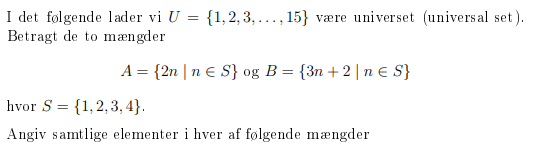
\includegraphics[width=1.0 \textwidth]{Reeksamen.PNG}
\begin{enumerate}[label=(\Alph*)]
\item $A
\\
$A = \big\{2,4,6,8\big\}
\\

\item $B 
\\
$B = \big\{5,8,11,14\big\}
\\

\item $A \cap $B 
\\
$A \cap $B = \big\{8\big\}
\\

\item $A\cup$B 
\\
$A\cup$B = \big\{2,4,5,6,8,11,13\big\}
\\

\item $A-B$
\\
A-B= \big\{2,4,6\big\}
\\

\item \overline{A}
\\ 
\overline{A} = \big\{1,3,5,7,9,10,11,12,13,14,15\big\}
\\

\end{enumerate}
\\



\end{document}
